%%%%%%%%%%%%%%%%%%%%%%%%%%%%%%%%%%%%%%%%%%%%%%%%%%%%%%%%%%%%%%%%%%%%%%%%%
% Template for a classical article
%%%%%%%%%%%%%%%%%%%%%%%%%%%%%%%%%%%%%%%%%%%%%%%%%%%%%%%%%%%%%%%%%%%%%%%%%
\documentclass[12pt,a4paper,notitlepage,onecolumn]{article}
%%%%%%%%%%%%%%%%%%%%%%%%%%%%%%%%%%%%%%%%%%%%%%%%%%%%%%%%%%%%%%%%%%%%%%%%%
\newcommand{\Author}{Fabio Zanini}
\newcommand{\Title}{FFPopSim: documentation for the SWIG interface}
\newcommand{\Keywords}{{FFPopSim}, {documentation}, {SWIG}}
%%%%%%%%%%%%%%%%%%%%%%%%%%%%%%%%%%%%%%%%%%%%%%%%%%%%%%%%%%%%%%%%%%%%%%%%%
\usepackage[english]{babel}
\usepackage[utf8x]{inputenc}
\usepackage{amsmath,amsfonts,amssymb,eucal,eurosym}
\usepackage{color}
\usepackage{framed}
\usepackage{minted}
\usepackage{graphicx}
\usepackage[font=small, format=hang, labelfont={sf,bf}, figurename=Fig.]{caption}
%\usepackage{cite}
%\usepackage{epigraph}
%\setlength{\epigraphwidth}{.55\textwidth}
%\setlength{\epigraphrule}{0pt}
%\usepackage{multirow}
%\usepackage[version=3]{mhchem}
%\usepackage{sagetex}
\usepackage[	colorlinks,linkcolor=red,citecolor=red]{hyperref}
\hypersetup{	pdfauthor={\Author}, pdftitle={\Title}, pdfkeywords={\Keywords}	}
%%%%%%%%%%%%%%%%%%%%%%%%%%%%%%%%%%%%%%%%%%%%%%%%%%%%%%%%%%%%%%%%%%%%%%%%%
\graphicspath{{./figures/}}
%%%%%%%%%%%%%%%%%%%%%%%%%%%%%%%%%%%%%%%%%%%%%%%%%%%%%%%%%%%%%%%%%%%%%%%%%
%\DeclareMathOperator\de{d\!}
%\newcommand{\comment}[1]{\textit{\textcolor{red}{#1}}}
%%%%%%%%%%%%%%%%%%%%%%%%%%%%%%%%%%%%%%%%%%%%%%%%%%%%%%%%%%%%%%%%%%%%%%%%%
\title{\Title}
\author{\Author}
\date{\today}
%%%%%%%%%%%%%%%%%%%%%%%%%%%%%%%%%%%%%%%%%%%%%%%%%%%%%%%%%%%%%%%%%%%%%%%%%
\begin{document}
%%%%%%%%%%%%%%%%%%%%%%%%%%%%%%%%%%%%%%%%%%%%%%%%%%%%%%%%%%%%%%%%%%%%%%%%%
\maketitle

%%%%%%%%%%%%%%%%%%%%%%%%%%%%%%%%%%%%%%%%%%%%%%%%%%%%%%%%%%%%%%%%%%%%%%%%%
\section{Introduction}
%%%%%%%%%%%%%%%%%%%%%%%%%%%%%%%%%%%%%%%%%%%%%%%%%%%%%%%%%%%%%%%%%%%%%%%%%
FFPopSim is a C++ library for population genetics with Python bindings. The
library was not written in pure Python for two reasons:
\begin{enumerate}
\item Efficiency;
\item To keep the possibility to control the code flow at low
level, by linking directly against the C++ library.
\end{enumerate}
The Python bindings are built via SWIG. In order to understand how they work
and possibly modify them, you need to understand abit of SWIG first.

\subsection{How does SWIG work?}
\begin{figure}
\begin{center}
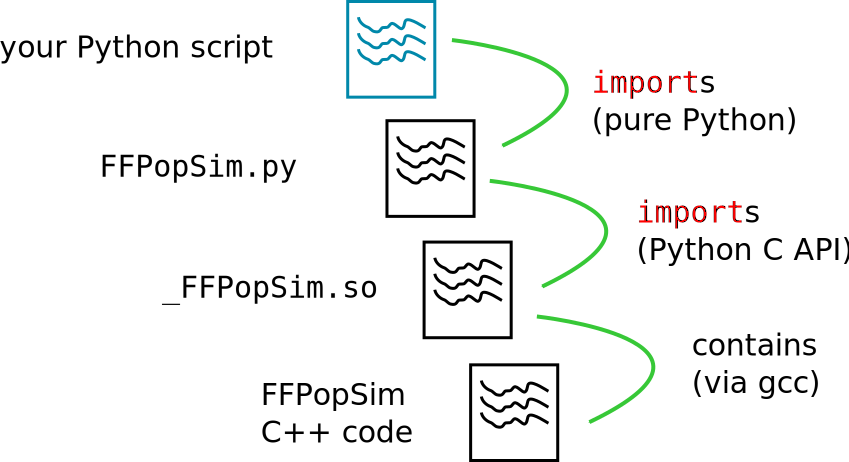
\includegraphics[width=0.7\linewidth]{schematic.pdf}
\caption{Levels and relationships in FFPopSim's SWIG C++ to Python interface.}
\end{center}
\end{figure}
SWIG takes two types of files in input:
\begin{enumerate}
\item {\color{blue}C++ header files}, ending in \texttt{.h};
\item {\color{red}interface files}, ending in \texttt{.i}.
\end{enumerate}
What SWIG does \textit{not} look at is the \texttt{.cpp} implementation files.
Whatever you write in those, it will never be part of the Python interface: only
the \textit{effects} of that code will be seen. For instance, if you do not
declare a function in the header file but implement it directly, that function
will be invisible to Python.

SWIG takes the {\color{blue}C++ header files} and makes a list of all constants,
variables, functions, classes, etc. Then, it runs over the {\color{red}interface
files} and checks whether any of those objects needs some special translation
rules; if so, it applies those rules. Finally, SWIG produces two output files:
\begin{enumerate}
\item a Python file, \texttt{FFPopSim.py};
\item a C++ wrap file, \texttt{FFPopSim\_wrap.cpp}.
\end{enumerate}
In order to get a complete Python module, you have to compile the generated wrap
file and link it against the C++ library into a \textit{shared library} file, named
\texttt{\_FFPopSim.so}. Note that this last step is \textit{not} part of SWIG
and can be achieved by different means: linking against a static version
(\texttt{FFPopSim.a}), recompiling the whole library together, using Makefile or
Python distutils and what not. Remember: in the end you are left with two files,
\texttt{FFPopSim.py} and \texttt{\_FFPopSim.so}, which constitute your Python
module. They are to be handled as a unit (same folder, etc.). Also, never try to
import \texttt{\_FFPopSim}, but only \texttt{FFPopSim}!

\subsection{{\color{red}Interface files}?}
C++ and Python are two very different languages. For instance, C++ has pointers,
explicit types, explicit pass by value or reference, the STL library; Python has
duck typing, no pointers whatsoever, a lot of builtin objects such as
dictionaries, sets, tuples.  Moreover, C++ and Python users expect different
\textit{styles} of programming, e.g. Python using properties in lieu of get/set
methods. For these reasons, a translation between C++ and Python cannot be fully
automatic and need some special rules. For example, we want to make sure that a
genotype, in C++ a \texttt{boost::dynamic\_bitset}, is converted into a numpy
array of bool, and vice versa. All these special rules are listed in the
interface files. In fact, you will spend most of your time writing such rules there.

%%%%%%%%%%%%%%%%%%%%%%%%%%%%%%%%%%%%%%%%%%%%%%%%%%%%%%%%%%%%%%%%%%%%%%%%%
\section{SWIG in FFPopSim}
%%%%%%%%%%%%%%%%%%%%%%%%%%%%%%%%%%%%%%%%%%%%%%%%%%%%%%%%%%%%%%%%%%%%%%%%%
\subsection{General architecture}
In FFPopSim, the C++ headers are in \texttt{src}, while the interface files in
\texttt{src/python}. The main interface file is \texttt{FFPopSim.i}. It does
three things:
\begin{enumerate}
\item It defines the name of the module, FFPopSim, and its docstring;
\item It includes standard pieces of SWIG code to convert STL vectors, maps,
strings, numpy arrays, etc;
\item It includes a few more FFPopSim-specific interface files for the various
parts of the library:
\begin{itemize}
\item \texttt{ffpopsim\_typemaps.i}: general recipes, called \textbf{typemaps};
\item \texttt{ffpopsim\_generic.i}: translates \texttt{ffpopsim\_generic.h}
\item \texttt{ffpopsim\_lowd.i}: translates \texttt{ffpopsim\_lowd.h}
\item \texttt{ffpopsim\_highd.i}: translates \texttt{ffpopsim\_highd.h}
\item \texttt{hivpopulation.i}: translates \texttt{hivpopulation.h}
\end{itemize}
\end{enumerate}
\begin{framed}
\noindent\textbf{Golden rule}: never touch the typemaps. Anything else you can modify pretty
easiliy once you get used to the code.
\end{framed}

In the next chapter, we'll see the
typical SWIG constructs used in FFPopSim: you can copy \& paste these snippets
to extend FFPopSim at will. Before that, however, a few more words of
explanation are needed.

\subsection{Interface files speak 3+ languages}
A typical chunk of an interface file looks like the following:
\begin{minted}{c++}
/* traits */
%feature("autodoc", "Number of traits (read-only)") number_of_traits;
const int number_of_traits;

%ignore trait;
void _get_trait(int DIM1, double* ARGOUT_ARRAY1) {
        for(size_t i=0; i < (size_t)DIM1; i++)
                ARGOUT_ARRAY1[i] = ($self->trait)[i];
}
%pythoncode {
\end{minted}
\vspace{-4ex}
\begin{minted}{python}
@property
def trait(self):
    '''Traits vector of the clone'''
    return self._get_trait(self.number_of_traits)
\end{minted}
\vspace{-4ex}
\begin{minted}{c++}
}
\end{minted}
This little part only is written in at least three languages: SWIG, C++, and
Python. Here's how to recognize them:
\begin{enumerate}
\item lines starting with an \% (percent sign) are SWIG commands (directives)
and provide a self-contained, special rule. In the example, we add a Python
docstring documentation to a class attribute, \texttt{number\_of\_traits};
\item lines with no special frame are C++ code that interfaces to the C++ library
as an external program. This code is present in the wrap file and eventually in
\texttt{\_FFPopSim.so};
\item lines within \texttt{\%pythoncode\{\}} or similar commands are pure
Python: they end up in \texttt{FFPopSim.py}.
\end{enumerate}
So here's the general rule: if you want to modify a rule (e.g. add a docstring,
ignore or rename a variable, etc.), use a SWIG directive; if you want to add
functions, classes, variables that are not speed critical, put them in a
\texttt{\%pythoncode\{\}} directive (like it is done for plot functions);
finally, if you need to access the C++ library at low level or to do efficient
loops, write C++ code. Unfortunately, putting three languages in a single file
makes it rather messy.

\subsubsection*{In depth: didn't you say 3+? Where's the 4th?}
NumPy. If you want to translate STL vectors into NumPy arrays instead of ad-hoc
objects or Python lists, you have to use stuff like:
\begin{minted}{c++}
void _get_trait(int DIM1, double* ARGOUT_ARRAY1) {
\end{minted}
The trick here are the two arguments, \texttt{DIM1} and \texttt{ARGOUT\_ARRAY1}.
They are used like normal input arguments in their C++ function but, in
addition, they have a special meaning for SWIG by virtue of the \texttt{numpy.i}
file. The latter makes sure that memory is allocated for the array before entering the
function and released by Python when the array is destroyed. In a sense,
lines like this are meaningful in 2 languages at the same time: C++ and the
\texttt{numpy.i} mini-language. If you think
this is horribly low level, think of the alternative: managing memory exchange
between C++ and Python ourselves (reference counting, garbage collection,
etc.)\dots not really exciting, uh?

\subsection{Example: add a class to FFPopSim}
Let us imagine you want to add a new subclass of \texttt{haploid\_highd} for the
HCV virus. After you have a working C++ code, proceed as follows:
\begin{enumerate}
\item decide where to put the \textit{declaration} of the new class. Check the
\texttt{Makefile} and the \texttt{setup.py} such that dependencies are fine
there. Let us assume you created a new header file called \texttt{hcv.h}:
\begin{minted}{c++}
#define HCV_STRAIN_ONE_A "1a"
#define HCV_STRAIN_TWO_A "2a"

class hcv : public haploid_highd {
public:
	hcv(int N=0, int rng_seed=0);
	virtual ~hcv();
	
	// strain of HCV
	string strain;
}
\end{minted}
\item Create an empty file in \texttt{src/python} called e.g. \texttt{hcv.i}.
\item Modify \texttt{FFPopSim.i} and include \texttt{hcv.h} (twice) and
\texttt{hcv.i} (once).
\item Open \texttt{hcv.i} and add \texttt{\%ignore} directives for all objects
in your header; check for compilation and runtime:
\begin{minted}{c++}
/* Interface file for hcv.h */
%ignore HCV_STRAIN_ONE_A;
%ignore HCV_STRAIN_TWO_A;
%ignore hcv;
\end{minted}
Of course, your class is
still invisible to Python, but at least you have not messed up the other
stuff!
\item Un-ignore constants, and add docstrings to them:
\begin{minted}{c++}
%feature("autodoc", "HCV strain 1a") HCV_STRAIN_ONE_A;
%feature("autodoc", "HCV strain 2a") HCV_STRAIN_TWO_A;
\end{minted}
\item Un-ignore the class, add a docstring to it, extend, add documentation for
the constructor, and ignore everything else:
inside:
\begin{minted}{c++}
%feature("autodoc", "FFPopSim class for HCV") hcv;
%extend hcv {
%feature("autodoc", "Constructor for the HCV class:

Parameters:
   - N: number of viruses in the population
   - rng_seed: seed of the random number generator
") hcv;
%ignore strain;
}
\end{minted}
\item Un-ignore the attribute of the class within the \texttt{\%extend\{\}}, add docstring,
check whether it works correctly:
\begin{minted}{c++}
%extend hcv {
...
%feature("autodoc", "HCV strain of this population") strain;
}
\end{minted}
\end{enumerate}
As you see, a big part of building SWIG interfaces is writing documentation.
This is crucial, because the same functions will work slightly differently in
Python from their C++ counterparts, and there is no Python code to look at for
help! When
writing docstrings, remember that the Python documentation is built using
reStructured text and Sphinx, so try to respect the conventions of those
programs (see the three spaces of indent under \texttt{Parameters:}?).

Now, if you got here, you're over the hardest! The following chapter provides
you with typical code snippets for your convenience.

%%%%%%%%%%%%%%%%%%%%%%%%%%%%%%%%%%%%%%%%%%%%%%%%%%%%%%%%%%%%%%%%%%%%%%%%%
\section{Reference snippets}
%%%%%%%%%%%%%%%%%%%%%%%%%%%%%%%%%%%%%%%%%%%%%%%%%%%%%%%%%%%%%%%%%%%%%%%%%
\subsection{Constants or read/write global variables}
Just add a docstring:
\begin{minted}{c++}
%feature("autodoc", "<Python documentation>") myconstant;
\end{minted}

\subsection{Read-only class attributes}
Python has no private attributes, nor get/set methods. You can still achieve the
same functionality with proterties:
\begin{minted}{c++}
%extend myclass {
...
%ignore myvar;
double _get_myvar() { return $self->myvar; }
%pythoncode {
\end{minted}
\vspace{-3ex}
\begin{minted}{python}
@property
def myvar (self):
    '''<YOUR DOCUMENTATION>'''
    return self._get_myvar()
\end{minted}
\vspace{-4ex}
\begin{minted}{c++}
}
...
}
\end{minted}
The trick here is that functions or variables starting with an underscore,
albeit public, are considered dangerous in Python, so the user should not touch
them. Moreover, the \texttt{\%ignore} directive only works at the Python level,
so our inline C++ function can still work (via the \texttt{\$self} trick).

\subsection{Classes}
You must include the following: a docstring for the class, a docstring for the
constructor, and \texttt{\%extend} directive, and string representation methods:
\begin{minted}{c++}
%feature("autodoc", "Class documentation") myclass;
%extend myclass {
%feature("autodoc", "Constructor documentation") myclass;
%feature("autodoc", "x.__str__() <==> str(x)") __str__;
%feature("autodoc", "x.__repr__() <==> repr(x)") __repr__;
const char* __str__() {
        static char buffer[255];
        sprintf(buffer, "...", ...);
        return &buffer[0];
}
const char* __repr__() {
        static char buffer[255];
        sprintf(buffer, "...", ...);
        return &buffer[0];
}
...
}
\end{minted}
See python \textbf{\_\_repr\_\_} and \textbf{\_\_str\_\_} for more details.

\subsection{Pointers}
SWIG can pass pointers to Python just right, but you cannot dereference them
from there, so usually dealing with bare pointers as input/output function
arguments is a bad idea. The typical solution is to write a C++ function that
works the same but without the pointer, e.g.:
\begin{minted}{c++}
%ignore myfunction;
%rename (myfunction) myfunction2;
vector <int> myfunction2 () {
// this function returns a vector instead of fiddling with
// C-style arrays
...
}
\end{minted}
\textbf{Note}: when working with objects, you sometimes want a function to
return a copy of the object. For instance, you do not want the na\"ive Python
user to modify the genealogy within \texttt{haploid\_highd}, for fear of damage.
Sometimes, however, you want to use pointers, to \textit{modify extant objects}. For
instance, if your population has an attribute called \texttt{location} which is
a struct and you want to modify it from Python, you will need a pointer to the
extant object, not a copy!

\subsection{Converting \texttt{std::<whatever>} into Python builtins}
Standard translation tables for STL objects can be less than optimal. If
efficiency is not an issue, you can use this trick:
\begin{minted}{c++}
%rename (_myfunction) myfunction;
%pythoncode {
\end{minted}
\vspace{-4ex}
\begin{minted}{python}
def myfunction(myargs):
    return list(_myfunction(myargs)) # or dict(...) for maps, etc.
\end{minted}
\vspace{-4ex}
\begin{minted}{c++}
}
\end{minted}
If you get an error because the object you have is not convertible into a
list/dict/..., check \texttt{FFPopSim.i} for the appropriate include statements
for the STL. If this is not sufficient, you might need a typemap. Good luck.

\subsection{Errors and exceptions}
The C++ part of FFPopSim uses two styles of error handling. Some functions
simply return nonzero values if an error has occurred (C style errors), other
functions \texttt{throw} actual C++ exceptions. Typically, the latter style is
employed in all cases where returning an \texttt{int} is not an option, e.g. for
class constructors (they return an instance of the class). How are errors
propagated to Python and handled there?

\begin{framed}
\noindent \textbf{Remember:} Error messages should be helpful for the user, not
generic or too low-level.
\end{framed}

\subsubsection*{C style error handling}
C style errors need no special translation, but look weird to Python users -- this
generates still another WTF moment each time. To make a better interface, you
can use the following recipe:
\begin{minted}{c++}
%exception myfunction {
  $action
  if (result) {
     PyErr_SetString(PyExc_RuntimeError,"Error in the C++ function.");
     SWIG_fail;
  }
}
\end{minted}
\textbf{Note}: \texttt{PyExc\_RuntimeError} is only one of the many possible
standard Python exceptions. Look at the Python C API website for more examples.

\noindent\textbf{Note}: the \texttt{if (result)} construct is very vaguely documented in
SWIG, hence this kind of code is probably fragile.

\subsubsection*{C++ style exceptions}
If the C++ library \texttt{throw}s an error that is not caught by Python, the
user won't be happy. Here's how you do that:
\begin{minted}{c++}
%exception myfunction {
        try {
                $action
        } catch (int err) {
                PyErr_SetString(PyExc_RuntimeError,"Error in the C++ function.");
                SWIG_fail;
        }
}
\end{minted}
Here we assumed the thrown exception is an \texttt{int} (this is the typical
case in FFPopSim), but it can be anything really.



%%%%%%%%%%%%%%%%%%%%%%%%%%%%%%%%%%%%%%%%%%%%%%%%%%%%%%%%%%%%%%%%%%%%%%%%%
%\bibliographystyle{plain}
%\bibliography{}
%%%%%%%%%%%%%%%%%%%%%%%%%%%%%%%%%%%%%%%%%%%%%%%%%%%%%%%%%%%%%%%%%%%%%%%%%
\end{document}
%%%%%%%%%%%%%%%%%%%%%%%%%%%%%%%%%%%%%%%%%%%%%%%%%%%%%%%%%%%%%%%%%%%%%%%%%

